\chapter{元素周期表：初步认识}\label{ch:g9:periodic-table-first-look}

几乎每间化学教室的墙上都挂着同一张图表：118
个方格，每个方格都标有一个符号和一个数字，排成行和列，
形状奇特——两侧是高耸的“塔”，中间有一处凹陷，
下方还有两行单独排列的方格。它于 1869 年首次绘制时，大约有
六十个方格，其中有几个空着。它的作者很有魄力，
敢于描述日后将填入这些空位的元素——
而他后来证明是对的。

\begin{recall}
元素是指原子序数 $Z$ 相同的一类原子，
即原子核中质子的数目（见\cref{ch:g9:inside-the-atom}）。
每种元素都有一个符号，由一个大写字母，有时加一个
小写字母组成（见\cref{ch:g7:atoms-and-molecules}）。铁、锌
和铝等金属能形成阳离子（见\cref{ch:g9:ions}）。
\end{recall}

\section{元素表}

\begin{definition}[元素周期表]\label{def:g9:periodic-table-first-look:periodic-table}
\emph{元素周期表}\index{元素周期表}列出所有化学
元素，按原子序数递增排列，即 $Z = 1$ 至 $Z = 118$，
并排成若干行，使性质相似的元素位于
同一列。
\end{definition}

\begin{definition}[周期与族]\label{def:g9:periodic-table-first-look:period}
元素周期表中的一行是一个\emph{周期}\index{周期}，共有
七个。一列是一个\emph{族}\index{族}，共有十八个，
从左到右编号为 1 至 18。表格下方印出的两行
属于第 6 和第 7 周期；另列出它们，只是为了让
表格保持较窄。
\end{definition}

\begin{omfigure}
\omperiodictable[colour=metals, legend=true, cell=0.86cm]

{\small 元素周期表。每个方格给出原子序数和
元素符号。颜色表示金属、准金属（介于金属与非金属之间的元素）和
非金属，按通常的分类方式划分。}
\end{omfigure}

\begin{method}[读懂元素周期表]\label{met:g9:periodic-table-first-look:read}
确定一种元素的位置，按下列步骤进行：
\begin{enumerate}
  \item 根据元素符号或原子序数找到它的方格；
  \item 其所在行给出周期，所在列给出族；
  \item 其颜色表明它是金属还是非金属。
\end{enumerate}
钠，\ce{Na}，$Z = 11$：第 3 周期，第 1 族，金属。氯，
\ce{Cl}，$Z = 17$：第 3 周期，第 17 族，非金属。
\end{method}

\section{金属与非金属}

\begin{definition}[金属与非金属]\label{def:g9:periodic-table-first-look:metal}
作为纯净物，\emph{金属}\index{金属}是指这样一类元素：新切开时有光泽，
导电、导热性良好，可以弯曲或锤打成形，
并且能形成阳离子。
\emph{非金属}\index{非金属}不具备这些性质：许多是气体，
如氧、氮、氯；固态的则暗淡、脆硬，
如硫和煤中的碳，它们倾向于形成阴离子，或在分子中共用
电子。
\end{definition}

\begin{proposition}[它们的位置]\label{prop:g9:periodic-table-first-look:where}
约五分之四的元素是金属；它们占据表格的左侧和
中部。非金属位于右上方，
氢单独位于左上角。沿二者的交界处，有少数元素
——硼、硅、锗、砷、锑、碲——具有
介于两者之间的性质，它们是准金属。
\end{proposition}

\section{性质相似的族}

\begin{proposition}[同一族的元素性质相似]\label{prop:g9:periodic-table-first-look:alike}
同一族的元素反应方式相似，所形成的
化合物也相似。锂、钠和钾位于第 1 族顶部，是
软金属，能与水反应并放出氢气；族中位置越靠下，反应
越剧烈。氟、氯、溴、碘位于
第 17 族，是有颜色的非金属，能与金属反应生成盐。
氦、氖、氩及第 18 族的其他元素几乎
不与任何物质反应。
\end{proposition}

\begin{inthelab}[锂、钠和钾与水的反应]
教师在安全挡板后，将一小块米粒大小的锂
投入一大碗水中：它轻轻地发出嘶嘶声。一小块
同样大小的钠在水面上快速游动，熔成一个银白色的
小球。钾立即燃烧，发出淡紫色火焰。三者都放出
氢气，并留下碱性溶液。
\end{inthelab}

\begin{safety}{\ghs[0.82cm]{GHS02}\ghs[0.82cm]{GHS05}}
% ledger: ghs:Na
钠：与水接触时会释放易燃气体，该气体可能
着火（GHS02）；可造成严重灼伤（GHS05）。钠须保存在油中，
仅由教师使用镊子夹取，并以极小的块进行操作。
\end{safety}

\section{门捷列夫的设想}

\begin{history}[门捷列夫留下的空位，1869--1886]
1869 年，德米特里·门捷列夫将当时已知的元素按
原子量递增的顺序排列——即原子的质量与
氢的质量相比较——并把性质相似的元素排在一起。
当规律需要时，他为尚未被发现的元素留下空位，
并于 1871 年描述了它们的性质：在硅的下方，有一种
“类硅”元素，其原子量约为 72。1886 年，
化学家克莱门斯·文克勒在一种银矿石中发现了锗，测得
其原子量为 72.3，并确认它就是那个空缺的元素。
镓（1875 年）和钪（1879 年）也填补了门捷列夫留下的空位。
\end{history}

\begin{omfigure}
\begin{minipage}[b]{0.32\linewidth}\centering
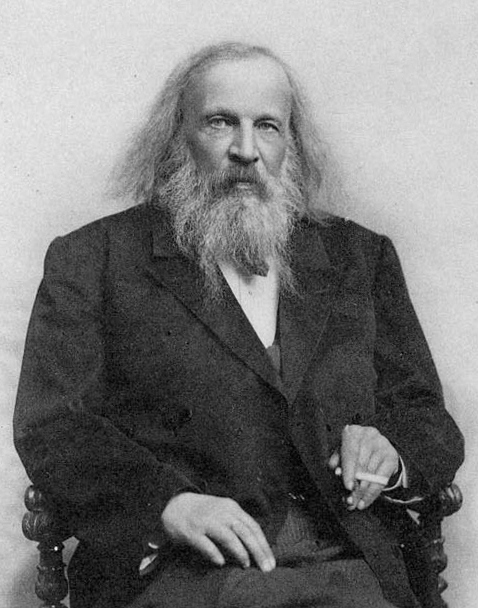
\includegraphics[width=\linewidth]{images/book1/mendeleev.jpg}

{\small 德米特里·门捷列夫（1834--1907）。}
\end{minipage}\hfill
\begin{minipage}[b]{0.6\linewidth}\centering
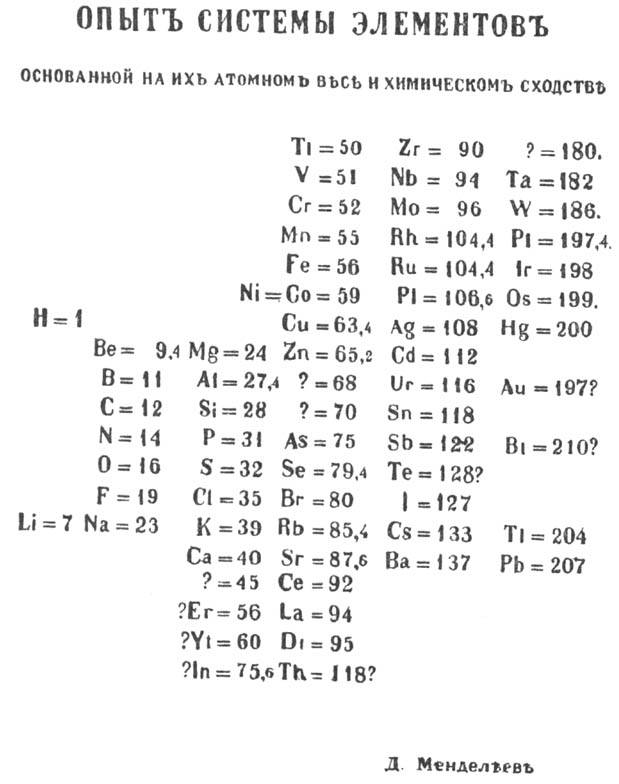
\includegraphics[width=0.85\linewidth]{images/book1/mendeleev-1869.jpg}

{\small 门捷列夫 1869 年绘制的俄文版元素表。在 Si $= 28$ 和
Al $= 27.4$ 旁，“? $= 70$”与“? $= 68$”两个空位
分别留给锗和镓。}
\end{minipage}
\end{omfigure}

\begin{remark}[按原子序数排序]\label{rem:g9:periodic-table-first-look:order}
门捷列夫按原子量给元素排序，为了使同族元素聚在一起，
不得不调换几对元素的位置，例如碲与碘，
如今元素周期表按原子序数排列，这一概念是后来才提出的，
因而不再需要这些调换。
\end{remark}

\section{练习}

\begin{exercise}[$\star$]\label{exo:g9:periodic-table-first-look:1}
元素在元素周期表中是按什么顺序排列的？
\end{exercise}

\begin{exercise}[$\star$]\label{exo:g9:periodic-table-first-look:2}
写出下列元素所在的周期和族：碳（$Z = 6$）、镁（$Z = 12$）、
氩（$Z = 18$）。
\end{exercise}

\begin{exercise}[$\star$]\label{exo:g9:periodic-table-first-look:3}
判断下列元素是金属还是非金属：铁、硫、铜、氧、铝、氯？
\end{exercise}

\begin{exercise}[$\star$]\label{exo:g9:periodic-table-first-look:4}
元素周期表中紧接在钠下方的是哪种元素？紧接在氯下方的呢？
\end{exercise}

\begin{exercise}[$\star\star$]\label{exo:g9:periodic-table-first-look:5}
利用元素周期表，写出第 4 周期第 2 族的元素，以及
第 2 周期第 15 族的元素名称。
\end{exercise}

\begin{exercise}[$\star\star$]\label{exo:g9:periodic-table-first-look:6}
为什么可以预料钾与钠一样，能与水发生反应？
\end{exercise}

\begin{exercise}[$\star\star$]\label{exo:g9:periodic-table-first-look:7}
某元素有光泽、能导电，并能形成离子 \ce{X^{2+}}。它是
金属还是非金属？请说明理由。
\end{exercise}

\begin{exercise}[$\star\star$]\label{exo:g9:periodic-table-first-look:8}
门捷列夫为什么要在表中留下空位？为什么这是他的表的优点，
而不是缺点？
\end{exercise}

\begin{exercise}[$\star\star$]\label{exo:g9:periodic-table-first-look:9}
观察门捷列夫 1869 年的元素表。他为碳和氧给出的原子量
各是多少？哪两个标有问号的空位，
出现在铝和硅的旁边？
\end{exercise}

\begin{exercise}[$\star\star$]\label{exo:g9:periodic-table-first-look:10}
第 2 周期和第 4 周期各有多少种元素？
\end{exercise}

\begin{exercise}[$\star\star\star$]\label{exo:g9:periodic-table-first-look:11}
氦、氖和氩几乎不与任何物质发生反应。它们位于
哪一族？根据这一性质，它们可以有什么用途？
\end{exercise}

\begin{exercise}[$\star\star\star$]\label{exo:g9:periodic-table-first-look:12}
镓位于铝的正下方，于 1875 年被发现。门捷列夫曾预言，
它的原子量应接近其相邻元素铝
（27.0）与铟（114.8）的平均值。计算该平均值。（镓：69.7。）
\end{exercise}

\section{问题：门捷列夫的空位}

\begin{problem}[{周末问题——由四个相邻元素预测一种缺失元素的
原子量}]
\label{pb:g9:periodic-table-first-look:1}
% ledger: aw:Si, aw:Sn, aw:Ga, aw:As, aw:Ge, mend:eka-si-aw, ge:winkler-aw
1871 年，门捷列夫预言了“类硅”元素的性质，它就是
硅下方缺失的那种元素。他的一个想法是，元素的性质
应介于其上方与下方、左侧与
右侧相邻元素的性质之间。目前测得空位四周四个元素的原子量为：
硅 28.1（上方）、锡 118.7（下方）、镓 69.7（左侧）、砷
74.9（右侧）。

\medskip
\noindent\textbf{第一部分——空位。}
\begin{enumerate}
  \item 利用本章的元素周期表，求出锗的原子序数、
        周期和族；锗是填补此空位的
        元素。
  \item 哪种元素位于锗的上方，哪种位于下方，哪种位于
        其左侧，哪种位于其右侧？
  \item 锗是金属、非金属还是类金属？
  \item 门捷列夫为什么预计缺失的元素会与
        硅相似？
\end{enumerate}

\medskip
\noindent\textbf{第二部分——平均值。}
\begin{enumerate}[resume]
  \item 计算空位上方元素与
        下方元素原子量的平均值。
  \item 计算空位左侧元素与
        右侧元素原子量的平均值。
  \item 上述两个平均值中，哪一个更接近
        锗的真实原子量 72.6？这可能是为什么？
  \item 门捷列夫在 1869 年的表中为此空位写下“? $= 70$”，
        他的估计偏差了多少？
\end{enumerate}

\medskip
\noindent\textbf{第三部分——预测。}
\begin{enumerate}[resume]
  \item 计算四个相邻元素原子量的平均值，
        保留一位小数。
  \item 1871 年门捷列夫预测其为 72；1886 年文克勒测得为 72.3。
        将结果与你算得的平均值作比较。
  \item 锗的发现为何使许多化学家确信
        门捷列夫的元素表是正确的？
  \item 请给出你的预测：根据四个相邻元素的平均值，
        给出类硅的原子量。
\end{enumerate}
\end{problem}
